\subsection{Reducing the velocity of executing a game}

\subsubsection{Problem analysis}

Because this game design enables some participants to be manipulated by the bot, once all participants are a bot and the whole program can be executed extremely fast and no interruption in it. 

And considering the visibility of when a token is placed on the board, it enables the player to know which token is being placed and be able to observe how is the game played by the bot. 

Thus, we use animation to complete this issue. However, there is a problem that how can allow the whole program to wait for the animation to be done and keep doing the following code. In other words, the animation should be implemented properly and in the meantime reduce the speed of the whole program running. The following analysis describes the possible solutions:

\paragraph{GUI animating} \mbox{}\\
Here is the first consideration. Once the animation is completed successfully, a way to inform the logic part that the animation works are done and also needs to be set up smoothly. 


\paragraph{Logic waiting} \mbox{}\\
Second, the logic part will not be interrupted or paused due to any conditions set. The noticeable issue is that once the GUI is doing animation, the logic part will execute continuous code and not wait for GUI animation.

\subsubsection{Realization analysis}
From the problem analysis above, it can easily be observed that an element to connect the logic part and GUI part is indispensable. Especially the characteristic of connecting two packages. In addition, there have some valid solutions described below: 

\begin{enumerate}
	\item\textbf{Callback}\\
A callback function can be called after the animation is done and coherent with the whole process of the code running. When the animation method is being called and executed, the GUI starts doing animation. But the logic part keeps running further down. And this callback function can lead the logic to wait for the animation to be done and follow up on the continuous work. 

	\item\textbf{Method reference}\\
The callback function is located at the logic part, and in order to let the GUI know which method should be called once the animation is completed. Hence, a method reference approach can be passed this callback function to the GUI part as a parameter.    
 
	\item\textbf{SetOnFinished}\\
The OnFinished function of the animation can sequence the whole process in a logical and reasonable direction. 
	

\end{enumerate}

\newpage
\subsubsection{Realization description}
According to the problem analysis above, the structure of implementing the callback function plays an important role. From Figure \ref{fig:StructureOfCallback} below, it can easily be comprehended that using animation to slow down the velocity of executing the program process is only demanded when the bot player is playing. However, no matter which turn is the bot or human player, the player hand token needs to increase and switch the turn player to the next. Therefore, those actions should be implemented in the callback function even if the combination of participants has human and bot, and the checking condition of whether the next player is a bot is also required to carry out here.   

Additionally, this call-back function can be passed as a parameter to an animation method by using method reference. And on the GUI, the run method of the Runnable Interface should be called to match with this callback function and invoked it. 

At last, the matched run method can be called in the onFinished method which is provided by the animation. This method will execute the callback method while the animation is entirely completed. 


\begin{figure}[h]
	\centering
	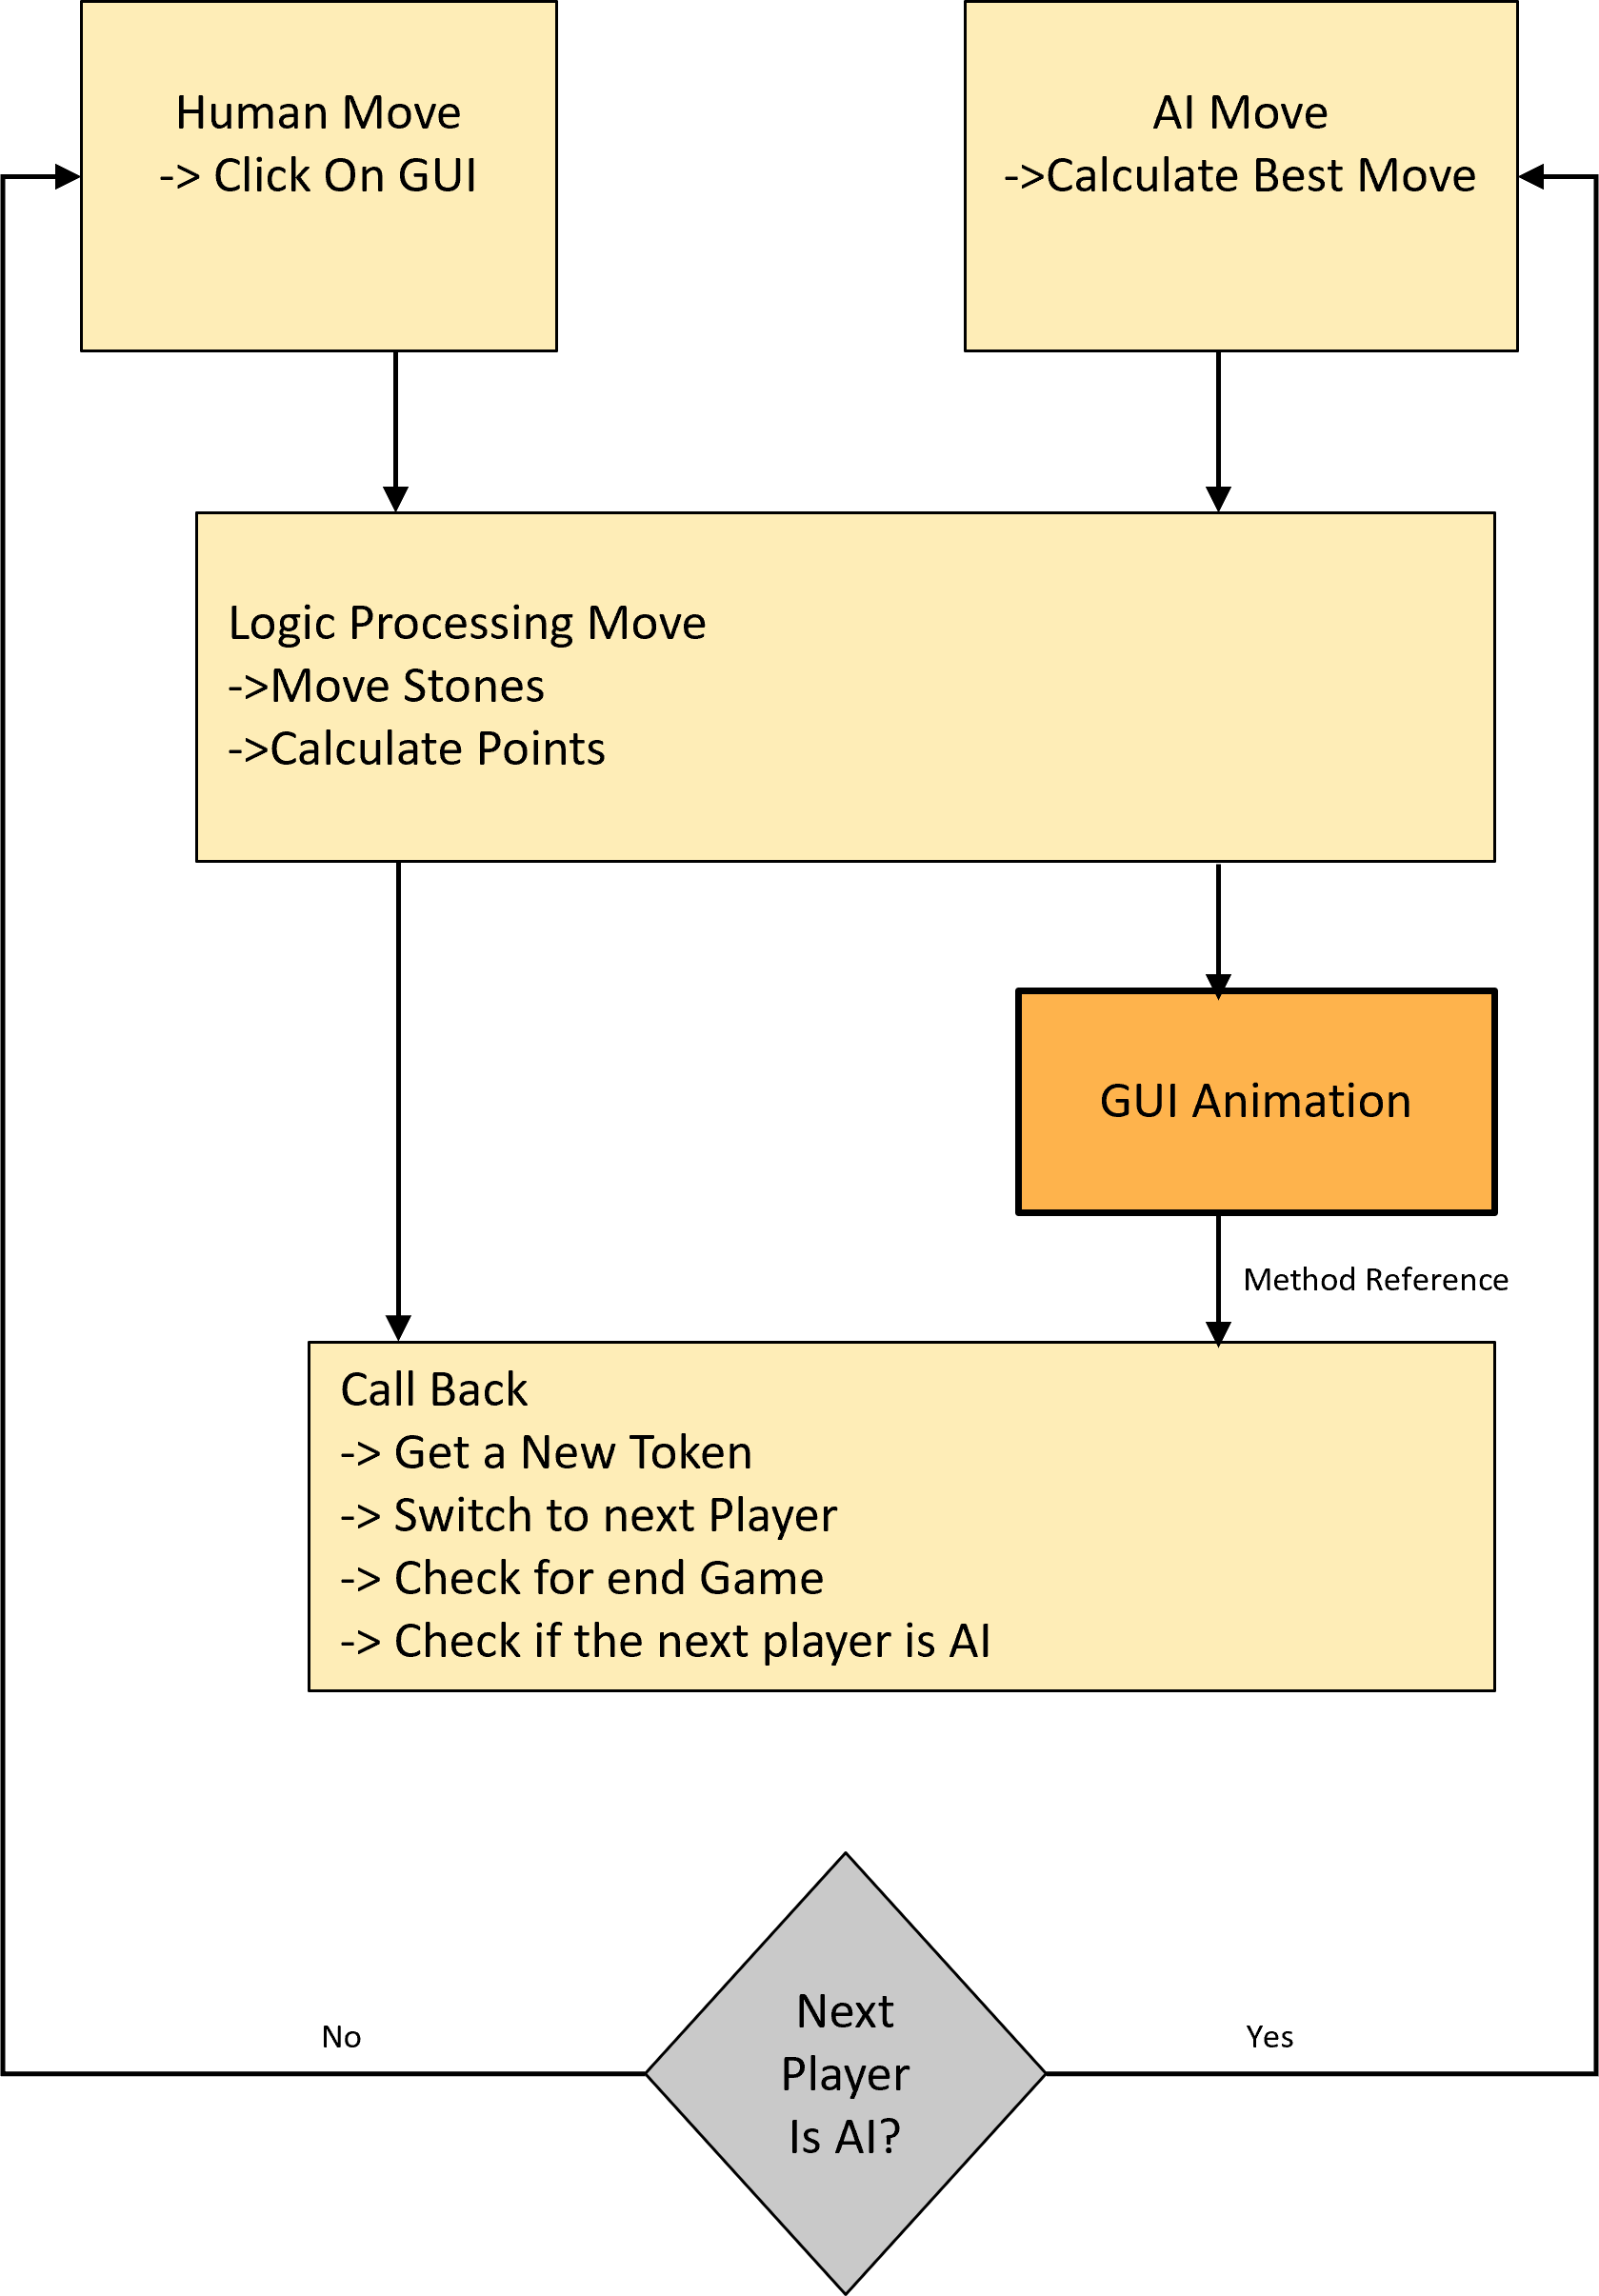
\includegraphics[width=0.6\textwidth]{image/StructureOfCallback}
	\caption{The Structure of callback function.}
	\label{fig:StructureOfCallback}
\end{figure}
